%
% [ SkAI Proposal  Template ]
%

\documentclass[11pt]{article}
\usepackage[utf8]{inputenc}
\usepackage{proposal}
% \usepackage{xcolor}
% \usepackage{epsfig}

\usepackage{graphicx}
\usepackage[dvipsnames]{xcolor}
% \usepackage{floatrow}
% \usepackage{minipage}
\usepackage[numbers,sort&compress]{natbib}
\setlength{\bibsep}{1.5pt}
\usepackage{aas_macros}

\usepackage{hyperref}
\hypersetup{
  colorlinks = true, % no ugly boxes around links
  urlcolor = [HTML]{0B5394}, % color for URLs
  linkcolor    = [HTML]{0B5394}, % color for internal links
  citecolor   = [HTML]{0B5394}, % color for citations
  breaklinks = true
}

\newcommand{\db}[1]{{\color{purple}[DJB: #1]}}
\newcommand{\am}[1]{{\color{olive}[AM: #1]}}

% ---  additional packages can be imported as needed

\usepackage{floatrow}
\usepackage[capitalise]{cleveref}
\usepackage{enumitem}
\usepackage{subcaption}

\begin{document}

% [ Research Proposal ]
%
% Discuss the significance of the proposed research to astronomy and AI. Please ensure following the text page limits, font size and layout guidelines as shared in the RfP.

\researchproposal

% \db{Regular proposals: up to 4 pages including figures}

\textbf{Learning the Functional Form of Dark Energy using Symbolic Regression}\\
% Deaglan Bartlett$^{1}$, Ayan Mitra$^{2}$,  Maxim Raginsky$^{2}$\\
%{\small
%$^{1}$\textit{Astrophysics, University of Oxford, Oxford, OX1 3RH, UK}\\
%$^{2}$\textit{University of Illinois Urbana--Champaign (SkAI Institute), Urbana, IL, USA}\\
%}\\
\underline{\textit{Vision}}

The Lambda Cold Dark Matter ($\Lambda$CDM) paradigm of cosmology, which has provided an extraordinarily successful description of the Universe over the past several decades, is increasingly under tension. Since the discovery of the accelerated expansion of the Universe in the  late 1990s \citep{Riess_1998,Perlmutter_1999}, the component of the cosmic energy budget responsible for this phenomenon (dark energy) has been assumed to take the form of Einstein’s cosmological constant, $\Lambda$. 
As the name suggests, the defining property of $\Lambda$ is that it is constant in time, corresponding to an equation of state $w=-1$ at all epochs. This assumption is the foundation of the $\Lambda$CDM model and has so far been broadly consistent with a wide range of cosmological observations.

However, the rapidly improving precision of cosmological data now allows this assumption to be tested in unprecedented detail. In particular, when one combines the latest measurements of baryon acoustic oscillations (BAOs) from the Dark Energy Spectroscopic Instrument \citep{DESI_2025_III} with observations of the cosmic microwave background (CMB) from Planck \citep{Planck_2018_VI} and Type Ia supernova (SNIa) distance measurements \citep{DES_2024}, indications of a possible time dependence in the properties of dark energy begin to emerge. While none of these datasets alone provides decisive evidence against $\Lambda$CDM, their joint analysis suggests mild but persistent deviations from a pure cosmological constant. If confirmed, such deviations would have profound implications for fundamental physics and cosmology.

The potential time evolution of dark energy is commonly encapsulated in its equation of state, $w(a)$, defined as the ratio of pressure to energy density as a function of the cosmic scale factor, $a$. 
In the $\Lambda$CDM model, $w(a)$ is strictly constant. In more general dark energy models, however, $w(a)$ can evolve with time \citep{Chevallier_2000}, reflecting underlying dynamics beyond a simple vacuum energy. 
Determining whether $w(a)$ departs from $-1$ and, if so, how it evolves is therefore one of the central goals of modern cosmology. 
If we are to understand the physical nature of dark energy, then we must go beyond testing specific parameter values and instead determine the functional form of $w(a)$ itself.

The aim of this proposal is to \textbf{infer this functional form directly from observational data}, without imposing strong theoretical priors on its shape. In other words, we seek to learn an analytic expression for $w(a)$ in a data driven manner, utilizing modern machine learning techniques for scientific discovery in fundamental physics. Rather than asking whether a particular model is consistent with the data, our approach asks what class of models the data themselves prefer.

This approach aligns closely with \textbf{Pillar 1} of this funding call (regular category). Rather than merely refining parameter constraints within a predefined cosmological model, our methodology \textbf{enhances inference} from cosmic survey data by \textbf{automatically searching over cosmological models} themselves in a principled, data driven manner. In doing so, this project has the potential not only to advance our understanding of dark energy, but also to establish a new paradigm for the use of machine learning in precision cosmology and fundamental physics more broadly.

\underline{\textit{Context and state of the field}}

\begin{figure}[hbt]
    \floatbox[{\capbeside\thisfloatsetup{capbesideposition={right,top},capbesidewidth=0.5\textwidth}}]{figure}[\FBwidth]
    {\caption{Equation of state, $w(a)$, for a theoretically motivated dark energy model (quintessence; black line, $\varphi$) compared to its best fit linear approximation for data sets from different probes (colored lines). Assuming this fixed functional form for $w(a)$ clearly does not fully capture the true behavior of dark energy \citep{Wolf_2023}. 
    This proposal will relax this overly restrictive assumption to prevent such biases.
    Figure from \citet{Wolf_2024}. \label{fig:wa_thawing}}}
    {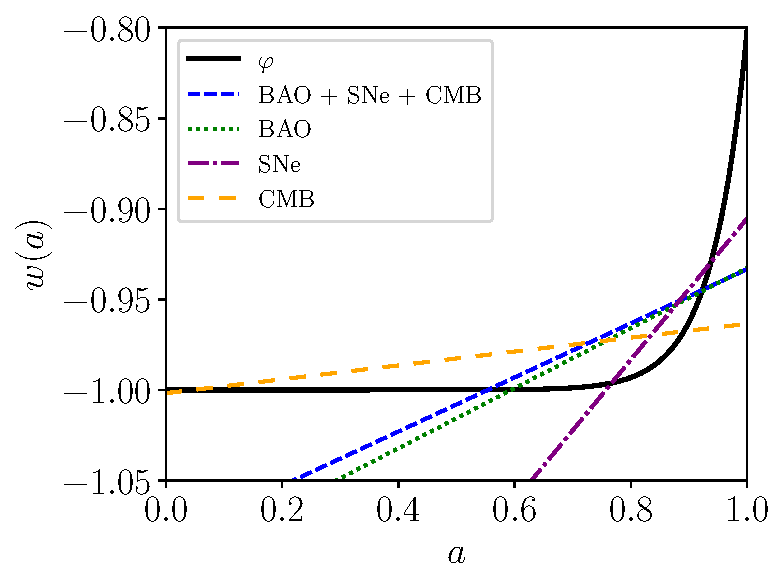
\includegraphics[width=0.38\textwidth]{figures/fitsw0wa_1.pdf}}
\end{figure}

Conventionally, an evolving dark energy equation of state is parametrized using simple, low dimensional ansatz, most commonly a linear function of $a$ \citep{Chevallier_2000,Linder_2002}. While such parameterizations are computationally convenient and have become standard in the field, they are not directly motivated by fundamental theory and may be overly restrictive. In particular, they implicitly assume smooth, linear evolution and may fail to capture more complex or unexpected behavior present in the data. As cosmological observations enter a precision era, there is a \textbf{growing risk that such restrictive assumptions could bias our inferences or obscure genuinely new physics}.
This is demonstrated in \cref{fig:wa_thawing}, where we see that linear fits to a well motivated dark energy model are very poor approximations, and thus could lead to incorrect conclusions about its dynamics.

To address this limitation, we propose to use the branch of machine learning known as symbolic regression (SR) \citep[for a recent review, see][]{Kronberger_2024} to learn a new functional form of $w(a)$ directly from observational data. SR searches the space of analytic expressions to identify compact, interpretable equations that best describe the data, rather than fitting parameters within a fixed model class. This makes SR uniquely well suited to the problem of discovering physical laws from data, as it produces explicit mathematical expressions that can be analyzed, tested, and embedded within theoretical frameworks.

Applied to cosmology, this approach has the potential to revolutionize our standard model by replacing the ``$\Lambda$'' in $\Lambda$CDM with a \textbf{data driven, AI discovered description of dark energy}. Crucially, the resulting model would remain \textbf{fully interpretable} and compatible with traditional cosmological inference pipelines, allowing rigorous statistical validation and comparison with existing theories.

To date, SR based scientific discovery has predominantly focused on the ``re-discovery'' of known physical laws from simulated or idealized data \citep{Schmidt_2009,Udrescu_2020,Lemos_2023}. While these studies have demonstrated the power of SR as a tool for interpretability and discovery, there have been relatively few applications aimed at uncovering genuinely new physics from real, noisy observational datasets. This proposal directly addresses that gap. By applying SR to state of the art cosmological observations, we aim to deliver what would be the \textbf{first major scientific breakthrough in fundamental physics enabled by SR}.

We propose to build on the Exhaustive Symbolic Regression (ESR) framework developed in \citet{Bartlett_2024}. 
ESR has been already successfully applied to cosmological analyses to learn the Hubble rate's evolution with redshift \citep{Bartlett_2024}, used to investigate the radial acceleration relation of galaxy dynamics, shedding light on claims regarding new laws of nature \citep{Desmond_2023}, utilized to find the optimal inflationary potential describing the dynamics of the early Universe \citep{Sousa_2024}, and leveraged to infer dark matter halo profiles from weak lensing data \citep{Martin_2025}.

ESR is uniquely well suited to this proposal because, unlike stochastic SR methods, it is \textbf{guaranteed to identify the optimal functional form} of the data up to a specified model complexity or expression length. 
This property is critical in the present context, where subtle features in cosmological data may encode physically meaningful departures from $\Lambda$CDM. 
In contrast, stochastic approaches to SR have been shown to be fallible in this regime, often failing to recover the correct functional form even when it lies within the search space \cite{Bartlett_2024,Kronberger_2024_inefficiency}.
For example, \cref{fig:esr_pareto} shows the performance of several well known SR algorithms 
(\textsc{PySR} \cite{cranmer2020discovering,pysr},
\textsc{DataModeler} \cite{DM},
\textsc{ffx} \cite{FFX},
\textsc{QLattice} \cite{QLattice}
and \textsc{operon} \citep{Burlacu_2020}) when fitting a standard normal curve containing data for $x>1$ only.
When plotting the error (mean squared error; MSE) against complexity (the number of symbols in the equation), the stochastic methods find either inacurate or complicated approximations, and cannot find the true generating function (which is at complexity 7). Only ESR is able to find this function.
By adopting an exhaustive approach, we therefore ensure that any inferred structure in $w(a)$ is driven by the data rather than by algorithmic artifacts or incomplete exploration of model space.

\begin{figure}[hbt]
    \floatbox[{\capbeside\thisfloatsetup{capbesideposition={right,top},capbesidewidth=0.4\textwidth}}]{figure}[\FBwidth]
    {\caption{Pareto front of solutions found by different SR algorithms when fitting a standard Gaussian lower truncated at $1$. By construction, ESR finds the optimum solution at a given complexity, whereas other methods have an unknown (high) probability of failing to find this. Figure adapted from \citet{Bartlett_2024}.\label{fig:esr_pareto}}}
    {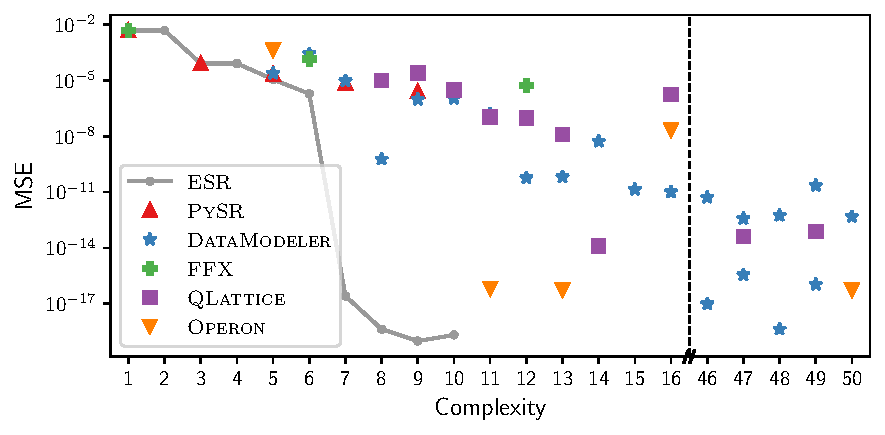
\includegraphics[width=0.55\textwidth]{figures/benchmark_pareto.pdf}}
\end{figure}

Model selection and comparison will be performed using information theory motivated metrics (description length \citep{Bartlett_2024}), allowing us to balance goodness of fit against model complexity in a principled and transparent manner. This is particularly important when searching over large spaces of analytic expressions, where overfitting and spurious structure can otherwise arise. In addition, we will \textbf{leverage recent advances in language model based techniques} \citep{Bartlett_2023} to preferentially select candidate models that resemble expressions commonly used in physics. By embedding inductive biases informed by the mathematical structure of physical theories, this approach will guide the SR towards models that are not only statistically favored, but also more likely to be physically reasonable and theoretically interpretable.

\underline{\textit{Objectives and methodology}}

% \db{Ensure covered: Include clear science deliverables, timelines, and metrics of success}

\textbf{1. SNIa based inference (months 0-6):} For this proposal, we will begin by interfacing ESR with SNIa based cosmological analyses, where the sensitivity to the late time expansion history makes them particularly well suited for probing the evolution of $w(a)$. Our initial focus will be on data and analysis frameworks relevant to the Vera C. Rubin Observatory Legacy Survey of Space and Time (LSST) \citep{LSST_2009}, which will deliver an unprecedented volume and quality of SNIa measurements. 
Using candidate dark energy models from ESR, we will develop software to compute the distant moduli of LSST SNIa for a proposed $w(a)$, and incorporate it within a likelihood to optimize both the free parameters in the dark energy model, as well as the other cosmological parameters.
The code will rank the ESR functions according to a modified computation of the description length, to incorporate the impact of the cosmological parameters and the language model priors introduced in \citet{Bartlett_2023}.
This will enable us to compute relative probabilities of the various dark energy models given the data, and thus obtain a definitive ranking of candidate $w(a)$ functions.
This stage of the project will allow us to develop, validate, and optimize the SR pipeline in a controlled and well understood setting.

\textbf{2. Multi probe inference (months 6-12):} Once we have a code which can reliably infer dark energy models given SNIa data, we will extend the approach to jointly inferring $w(a)$ from SNIa and BAO measurements. Combining these complementary probes will significantly enhance sensitivity to dark energy evolution while helping to break parameter degeneracies and reduce systematic biases. Crucially, the SR framework naturally accommodates such joint analyses, enabling the discovery of functional forms that are simultaneously consistent with multiple cosmological observables.

\textbf{3. Pipeline validation (throughout):} Throughout the project, we will \textbf{extensively test our pipeline using survey realistic mock catalogs} \citep{Mitra_2023,Mitra_2025}. These mocks will allow us to rigorously validate the robustness, accuracy, and interpretability of the inferred models under realistic noise, selection effects, and systematic uncertainties. Only after demonstrating reliable performance on these mock datasets will we apply the method to real observational data, ensuring that any inferred departures from $\Lambda$CDM are robust and reproducible.
There are two clear metrics of success which we will use to validate our pipeline:
\begin{enumerate}[
    topsep=0pt,
    partopsep=0pt,
    parsep=0pt,
    itemsep=0pt,
    label=\alph*)]
    \item \textit{Parameter regression:} If one knows the functional form of the dark energy model but not its free parameters, then one should be able to infer these correctly using the chosen likelihood model. For a range of dark energy models and for multiple mock realizations, we will ensure that we obtain unbiased estimates of these parameters with correctly calibrated uncertainties. This will test our likelihood model.
    \item \textit{Symbolic regression:} Once we have validated our likelihood, we will ensure that mocks made with given dark energy models can be rediscovered by our pipeline. If a model is not rediscovered, we will identify how many SNIa would be required to rediscover it (since more complicated models need more data to have sufficient evidence to be discovered). This stage is crucial to identify the limitations of current datasets and forecast the discovery potential of future data.
\end{enumerate}
Much of the infrastructure for creating these mocks for the pure supernova inference has already been produced  \citep{Mitra_2023,Mitra_2025} for $\Lambda$CDM cosmologies, so we will begin by adapting these to alternative dark energy models to test Objective 1 of this proposal.
Once these changes have been made, we will produce a new mock generation pipeline to also incorporate the additional probes required for Objective 2. As such, this objective will be continually worked on throughout the project. 

% \db{Make clear what data we plan to use once the pipeline is validated and when it is ready}

If this programme is successful, we will pursue future funding opportunities to extend the framework to incorporate next generation CMB survey data and to address a broader class of cosmological inference problems. These include possible applications such as redshift distance relations without explicitly assuming FLRW geometry, bias modelling in galaxy clustering, phenomenological descriptions of modified gravity, and supernova standardisation beyond the Tripp relation etc. While diverse in application, these problems are united by a common underlying challenge namely the absence of well motivated or unbiased functional forms which SR is uniquely positioned to address.

By providing a common and interpretable model discovery language across these settings, this expansion naturally enables a fully joint, self consistent analysis of SNIa, BAO, and CMB observations within a unified SR framework. Ultimately, the project aims to deliver a robust, user friendly model discovery tool whose underlying methodology is broadly applicable to cosmology and to other areas of the natural sciences facing similar challenges of functional form discovery,  \textbf{highlighting the broader relevance of SR as a foundational methodology for interpretable scientific inference.}





\underline{\textit{Outputs and impact}}

In accordance with the aims of the funding call, this proposal will produce \textbf{software suites} to automatically find dark energy models given cosmological data. We will make all such software publicly available via GitHub, providing examples and tests to ensure ease of use by the community.
To validate our pipeline, we will produce many survey realistic mock \textbf{datasets}, which again will be made publicly available through platforms such as Zenodo. 
% \db{@Ayan is that ok?} \am{this is ok}
Finally, we expect that the AI discovered dark energy \textbf{model} will be of great use for the community due to its robust data driven discovery and its analytic form will make it easy to integrate into future cosmological pipelines or for further theoretical  study.

Beyond its immediate cosmological applications, this project also constitutes a foundational contribution to artificial intelligence. The SR framework we will develop is broadly applicable to any scientific domain in which discovering analytic structure from data is essential. Its scope extends far beyond dark energy, offering a general, interpretable model discovery tool that could transform fields ranging from astrophysics to climate science and materials physics. As such, this work has the potential to represent a genuine breakthrough in AI driven  inference of fundamental science, demonstrating how machine learning can move beyond black-box prediction to the discovery of new, human interpretable physical laws.

% \db{What we plan to output here. ``Develop software suites, models, and datasets that can be used and adopted by the scientific community.'' }

\underline{\textit{Requested resources}}
We are requesting support for a junior researcher (e.g. a graduate student) to carry out this work, as the scope and structure of the project are well matched to this level. The project requires sustained development of a novel analysis pipeline, close interaction with real and simulated cosmological datasets, and iterative methodological refinement, which are activities that are ideally suited to a researcher working under structured mentorship. In turn, this work will be highly beneficial to the researcher, providing rigorous training at the intersection of AI and observational astrophysics, hands on experience with interpretable machine learning and large survey data, and opportunities to publish, present, and develop independence as an interdisciplinary researcher.


\pagebreak

\bibliography{main}
\bibliographystyle{nsf_limit5authors}

\clearpage

% [ Mentoring Plan ]
%
% This section should consist of text only (no figures).
% There is a limit of one page of printed text.

\mentoringplan
The objective of this mentoring plan is to train a junior researcher (e.g. graduate student) to operate at the interface of foundational AI and observational astrophysics. The trainee will gain hands on experience in developing and applying interpretable, physics informed machine learning methods (particularly SR), for discovering analytic models from complex observational data. By the end of the project, the trainee will be expected to independently lead interdisciplinary research at the intersection of AI and the physical sciences, in alignment with the mission of the SkAI Institute.

To achieve these goals, mentoring will be structured around regular group sessions with the full team, including Lead PI Prof. Raginsky, to discuss progress, troubleshoot challenges, and integrate feedback. In the first six months, the trainee will focus on supernova based inference (Objective 1), gaining proficiency in ESR software integration and cosmological data handling through hands on coding tasks, such as adapting mock catalogs \citep{Mitra_2023,Mitra_2025} for dark energy models. Dr. Bartlett will provide targeted training on SR algorithms and physics informed priors \citep{Bartlett_2023}, while Dr. Mitra will guide the application to LSST relevant SN datasets, ensuring the trainee develops skills in likelihood optimization and model ranking. By months 6-12, the trainee will lead aspects of multi probe inference (Objective 2), including pipeline validation with BAO data, fostering independence through assigned sub tasks like generating new mocks and analyzing results. Throughout, we will incorporate professional development opportunities, such as co-authoring publications, presenting at SkAI workshops or conferences (e.g., AAS meetings), and attending  seminars on AI in science, to build the trainee's network and communication skills.


 We are dedicated to fostering an inclusive research environment and will prioritize recruitment of candidates from underrepresented groups in STEM fields, consistent with SkAI’s commitment to diversity and equity. Furthermore, the trainee will be expected to engage actively in SkAI wide seminars, workshops, and cross institutional collaborative events including those organized by our team on SR and will be strongly encouraged to co-lead or contribute to tutorials and training sessions. These activities will cultivate essential communication, presentation, and leadership abilities while building  professional networks across SkAI core and satellite institutions.




\pagebreak

% [ Additional Project Personnel Funded by Other Sources ]
%
% This section should consist of text only (no figures).
% The text should not exceed 0.5 page.

\teaminfo
% \vspace{15em}
% enter information about team members not funded by SkAI
Dr. Deaglan Bartlett (University of Oxford): Dr. Bartlett is the primary scientific lead and developer of the ESR framework. As a \textbf{Schmidt AI} in Science Fellow, he provides the foundational AI expertise that powers this proposal, including the development of physics informed priors and the integration of language models for symbolic discovery. He will lead the algorithmic development and the optimization of the symbolic search space. His participation is fully funded by his home institute, Oxford University.

Dr. Ayan Mitra (UIUC): As a SkAI Affiliate PI, Dr. Mitra will co-lead the overall project, and coordinate the ESR  pipeline with cosmological datasets, and oversee the  research progress of the funded student.


Lead PI Prof. Maxim Raginsky (UIUC): While he will serve as the lead PI, his primary effort is supported by his faculty position at UIUC.




% [ SkAI Engagement Activities ]
%
% This section should consist of text only (no figures), of approximately 1/2 page of printed text.
\engagement
% enter information about how the team will engage with SkAI activities
We will contribute to the SkAI community through a multi disciplinary engagement strategy:
\begin{enumerate}[
    topsep=0pt,
    partopsep=0pt,
    parsep=0pt,
    itemsep=0pt,]
    \item  Workshops and Seminars: We will organize workshops on SR providing SkAI researchers with the tools to implement AI driven interpretable discovery in their own research domains.  Dr. Bartlett will lead the technical tutorials, leveraging his experience of delivering similar training for Microsoft Industry Solutions and his role in organizing the \href{https://royalsociety.org/science-events-and-lectures/2025/04/symbolic-regression/}{international Royal Society discussion meeting} on ``Symbolic Regression in the Physical Sciences''. These efforts will be technically supported by Dr. Mitra and Prof. Raginsky’s whose expertise in information-theoretic foundations will be useful. Additionally, we propose to use Prof. Raginsky's  role as a SkAI Core Member to facilitate interdisciplinary seminars that connect our project’s breakthroughs with the broader  AI communities. These sessions will focus on moving beyond ``black box'' AI models toward the human interpretable physical laws discovered using AI.
    \item Integrated Mentoring: We will actively participate in the \href{https://skai-institute.org/education/educational-programs/}{SkAI SEED program} by hosting undergraduate researchers, providing them with a unique ``theory to application'' environment. Students would experiment with the implementation of new dark energy models or data sets into the pipeline to test code or extend
    to new datasets. Students will therefore gain hands on exposure to the real world implementation of interpretable AI algorithms by applying the SR  framework to cosmological discovery. With further possibility that these researchers could be integrated into the research groups at UIUC (or other SkAI satellite institutes) later on.  
    \item Software Curation and Outreach: In alignment with SkAI’s open science mission, our team will release a curated software suite with thorough documentation and a library of AI discovered dark energy models.
%\item Seminar Series on Foundational AI: 
\end{enumerate}


% \db{Some ideas:}
% {
% \color{purple}
% \begin{itemize}
%     \item Workshops: Deliver a symbolic regression workshop/training activity. DB has experience running such training for Microsoft Industry Solutions 
%     \item Meetings: DB experience organizing SR workshop (discussion meeting at The Royal Society on `Symbolic Regression in the Physical Sciences' - multi-discipline). Could organize a similar event in the US since the RS one was in Europe
%     \item Summer students: Could implement new DE models or data sets into pipeline to test code or extend to new datasets
% \end{itemize}
% }



\end{document}
